\documentclass[jou,apacite]{IEEEtran}
\usepackage{graphicx}
\usepackage{amsfonts}
\usepackage{amsthm}
\usepackage{tabu}
\usepackage{amssymb}
\usepackage{mathtools}
\usepackage{relsize}
\graphicspath{ {./images/} }
\setlength\parindent{0pt}

\title{Scala - A Powerful and Scalable Function-Objective Programming Language}

\author{Troy Hu and Benjamin Killeen} % alphabetical by last name

\begin{document}
\maketitle    
\begin{abstract}
Insert abstract here.
\end{abstract}                     

\section{Introduction}
\label{sec:intro}

During the mid 2000s, progress in developing component software was slow, which the researchers believed to be because existing languages had little support for component abstraction and composition. Some examples include statically typed languages such as Java and C\#. In response to this lack of progress, Odersky et al. designed and implemented Scala in order to develop better language support for component software. As the researchers put it, components ``are simply software parts which are used in some way by larger parts or whole applications. Components can take many forms; they can be modules, classes, libraries, frameworks, processes, or web services." At the same time, they envisioned their language as eventually being widely adopted. 


The researchers achieved their goals by focusing on two areas: 
\begin{itemize}
\item Developing scalable mechanisms for abstraction, composition, and
  decomposition. Through this focus, they made their language more scalable
  than existing languages such as Java. I.e., small and large components of
  component software can be expressed with the same concepts.
\item Combining functional programming and object-oriented
  programming. Odersky et al. decided to combine these two programming
  paradigms in order to prove better scalable support for software
  components.
\end{itemize}
We now describe on a high-level how Scala achieves its goals of providing
good support for component software and encouraging mass adoption.

\subsection{High-Level Design}
\label{sec:high-level-design}

In order to encourage adoption by software developers, Scala's syntax is very similar to Java's and C\#'s. In fact, Scala is able to work and interact with components coded in Java and C\#. However, remember that Java and C\# are suboptimal languages for supporting component software. Thus, in order to improve component support over Java and C\#, Scala discards or modifies some their existing conventions. For example, Figure 1 demonstrates a simple program (CITE THIS) that prints out options provided in the command line.
\begin{figure}[h]
  \centering
  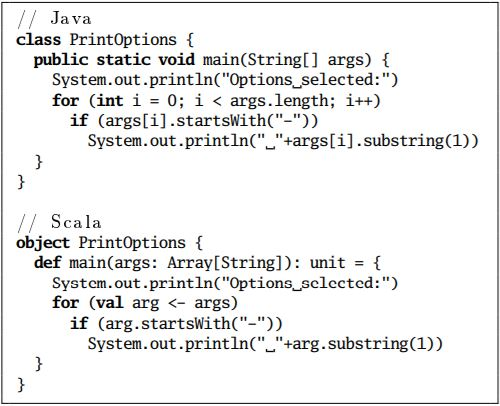
\includegraphics[width=\columnwidth]{exampl1.JPG}
  \caption{Figure 1. Notice how Scala's general syntax and structure are similar
    to Java's. At the same time, there are some visible differences, e.g., unit
    is returned in the Scala implementation instead of void in the Java
    implementation. (CITE THIS IMAGE FROM OVERVIEW PAPER.)}
  \label{fig:example}
\end{figure}

Large parts of Scala's typing system are unique to the language. Scala's abstract type definitions and path-dependent types utilize $\nu$Obj Calculus (See Section III). Additionally, Scala implements modular mixin composition which combines the advantages of mixins and traits. Traits in Scala are essentially the equivalent of abstract classes in Java while mixins are classes/traits in which other non-child traits can draw methods from. \\\\
Scala also has a uniform object model. That is, every value is an object and
every operation is a call to a method. For example, the boolean “true” itself is
an object (S singleton object, in fact. See Section II for definition of
singleton object). At the same time, Scala includes functional programming
aspects such functions being first-class values (i.e. functions can be passed as
values) and pattern matching. For pattern matching specifically, Scala allows
objects themselves to be decomposed. This language also implements powerful and
novel abstraction concepts for types and values. For example, unlike Java
abstract classes, traits can include method implementations or fields.

% 3. related work
\section{Related Work}
\label{sec:related-work}


% 2. Technical summary: Killeen
\section{Interesting Technical Details}
\label{sec:interesting-tech}

% singleton objects

% unified object model

% pattern matching in an object oriented setting

% Abstraction:
% - subtypes and polymorphism
% -

% Traits and classes:
% A trait do encapsulate state. They just define methods or variables that you
% have to have but don't provide instantiated values for those.

% Classes require implementations or values for everything.

% Views in Scala implement something close to SML's signatures or Haskell's
% typeclasses.

% Multiple inheritance with mixins.

% 4. report on peano arithmetic calculator.
\section{Engagement: Peano Arithmetic Calculator}
\label{sec:engag-peano-arithm}

% 5. should encapsulate discussion of current status
\section{Discussion}
\label{sec:discussion}

\section{Current Status of Work}
After 15 years, Scala has been regularly updated and is currently at stable
release version 2.12.8. Over this period, the core principles of Scala have
remained the same. Scala has achieved widespread adoption in the industry with
companies such as Twitter and Apple utilizing the language. Moreover, Scala has
both a large academic and non-academic user base. The language is often cited or
used in computer science research. In addition, Scala's user community is
thriving. there exist chatrooms, subreddits, and research conferences devoted
entirely to Scala. Numerous libraries, tutorials, and guides are run and
maintained by the community. The main community page can be found at:
https://www.scala-lang.org/community/. A detailed, updated, and easy to read
documentation can be found at: https://docs.scala-lang.org/. Finally, there are
dedicated installers/installation guides for all operating systems at:
https://www.scala-lang.org/download/.


\bibliographystyle{IEEEtran}
\bibliography{scala_project}

\end{document}

%%% Local Variables:
%%% mode: latex
%%% TeX-master: t
%%% End:
